%//==============================--@--==============================//%
\subsection[5.1 Circuitos Integrados NMOS e CMOS]{\hspace*{0.075 em}\raisebox{0.2 em}{$\pmb{\drsh}$} Circuitos Integrados NMOS e CMOS}
\label{subsec:circuitos-integrados-NMOS-e-CMOS}

Nos circuitos, integrados as resistências ocupam maior área relativamente aos transístores; apesar de serem concebíveis resistências de valor elevado e área reduzida, estas apresentam tolerâncias muito elevadas. É então desejável diminuir o número de resistências no circuito, ou removê-las por completo. Nos circuitos com BJTs, isto não é possível, somente com \textbf{tecnologias MOS} (modo de funcionamento óhmico na região de tríodo). 

\begin{itemize}[leftmargin=*]
    \item A \textbf{tecnologia} mais \underline{simples} e \underline{barata} é a \textbf{NMOS}, que, na sua versão mais elementar, apenas permite realizar transístores NMOS de reforço, e, numa versão mais avançada, permite realizar transístores NMOS de reforço e de depleção. (A tecnologia PMOS, utilizada nos primórdios, foi substituída por NMOS, porque nesta os transístores conseguem menores dimensões retendo um nível de funcionamento semelhante.)
    
    \item A \textbf{tecnologia CMOS} é \underline{mais evoluída}, permite realizar transístores NMOS e PMOS, ambos de reforço; a letra C refere-se à existência de dispositivos \textbf{complementares}.
\end{itemize}

%//==============================--@--==============================//%
\subsubsection[5.1.1 Circuito base de cada tecnologia MOS]{$\pmb{\rightarrow}$ Circuito base de cada tecnologia MOS}

%//==============================--@--==============================//%
\paragraph[5.1.1.1 Tecnologia NMOS com transístores de reforço]{$\pmb{\star}$ Tecnologia NMOS com transístores de reforço}\mbox{}\\[4pt]
Na tecnologia NMOS com transístores de reforço, o circuito base é o \textbf{inversor NMOS com carga de reforço}. Podemos considerar que este circuito tem origem no andar de fonte comum, em que a resistência de carga é substituída pelo transístor $M_2$.

\begin{figure}[H]
    \centering
    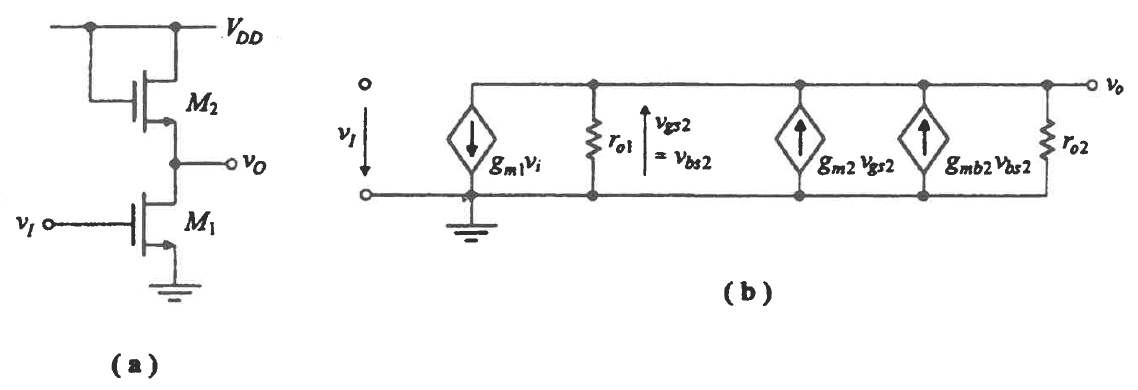
\includegraphics[width=0.6\linewidth]{img/5/inv-NMOS-carga-ref.png}
    \caption{Inversor NMOS com carga de reforço \cite{medeiros:CTBM}}
    \label{fig:inv-NMOS-carga-ref}
\end{figure}

\vspace{-0.75em}
\noindent O transístor $M_2$ tem a porta ligada ao dreno ($v_{GS2} = v_{DS2}$), e por isso está saturado
$$
     i_{D2} = k_2 (V_{DD} - v_O - V_{t2})^2 \quad \text{(resistência não-linear)}
$$
\noindent O funcionamento como inversor resume-se da seguinte forma:
\begin{itemize}[leftmargin=*, nolistsep, label=\raisebox{-0.1em}{\ding{43}}]
    \item $v_I \to \text{HIGH}$, $M_1$ está cortado, $i_{D1} = i_{D2} = 0$, o que resulta em $v_O = V_{DD} - V_{t2}$;
    \item $v_I \to \text{LOW}$, $M_1$ conduz, o que faz $v_O$ passar para o nível baixo.
\end{itemize}

\begin{mdframed}
    \noindent O circuito também se pode utilizar como amplificador: $A_v \approx -\frac{g_{m1}}{g_{m2} + g_{mb2}}$, dado que $r_{o1}$ e $r_{o2} \gg g_{m2}$, e estão em paralelo. 
    
    Se se desprezar o efeito de corpo, $A_v \approx -g_{m1}/g_{m2} = -\sqrt{k_1/k_2} = -\sqrt{\frac{(W/L)_1}{(W/L)_2}}$

    \vspace{0.5em}
    \noindent Como as dimensões $W$ e $L$ dos transístores têm um valor mínimo, para se evitarem grandes dimensões, o ganho de tensão não pode exceder um valor na ordem de 10.
\end{mdframed}

%//==============================--@--==============================//%
\paragraph[5.1.1.2 Tecnologia NMOS com transístores de reforço e de depleção]{$\pmb{\star}$ Tecnologia NMOS com transístores de reforço e de depleção}\mbox{}\\[4pt]
Neste caso, o circuito base é o \textbf{inversor NMOS com carga de depleção}. Podemos, novamente, considerar que este circuito se obtém através do andar de fonte comum, em que a resistência de carga é trocada por uma resistência não-linear (transístor de depleção). Nesta configuração, a porta está ligado à fonte.

\begin{figure}[H]
    \centering
    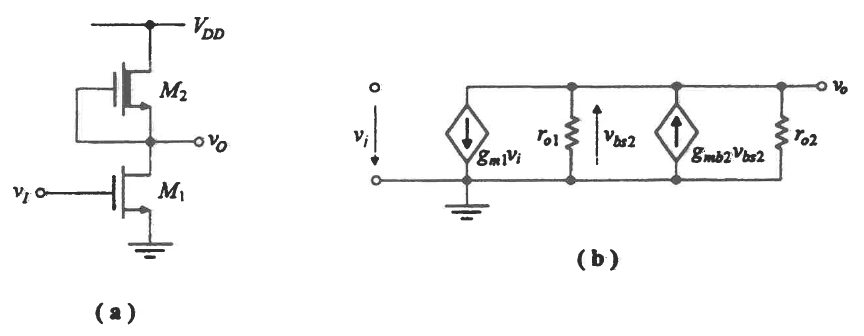
\includegraphics[width=0.6\linewidth]{img/5/inv-NMOS-carga-dep.png}
    \caption{Inversor NMOS com carga de depleção \cite{medeiros:CTBM}}
    \label{fig:inv-NMOS-carga-dep}
\end{figure}

\vspace{-0.75em}
\noindent O funcionamento como inversor resume-se da seguinte forma:
\begin{itemize}[leftmargin=*, nolistsep, label=\raisebox{-0.1em}{\ding{43}}]
    \item $v_I \to \text{HIGH}$, $M_1$ está na zona de tríodo e $M_2$ fica saturado, $v_O \to \text{LOW}$;
    \item $v_I \to \text{LOW}$, $M_1$ está cortado, o que faz $i_{D2} = 0$, $M_2$ está na zona de tríodo com $v_{DS2} = 0$, e portanto, $v_O = V_{DD}$, que constitui o nível alto.
\end{itemize}

\begin{mdframed}
    \noindent O circuito pode funcionar como amplificador se $M_1$ e $M_2$ estiverem em saturação.

    O ganho de tensão é aproximadamente $A_v = -g_{m1}/g_{mb2}$, e como $g_{mb2} = 0.1$ a $0.3\, g_{m2}$, comparando com a versão anterior, temos um ganho significativamente superior. (No passado, este circuito foi também utilizado como andar amplificador.)
\end{mdframed}

%//==============================--@--==============================//%
\paragraph[5.1.1.3 Tecnologia CMOS]{$\pmb{\star}$ Tecnologia CMOS}\mbox{}\\[4pt]
Tal como os circuitos anteriores, o \textbf{inversor CMOS} pode ser utilizado como inversor lógico ou amplificador.

\begin{figure}[H]
    \centering
    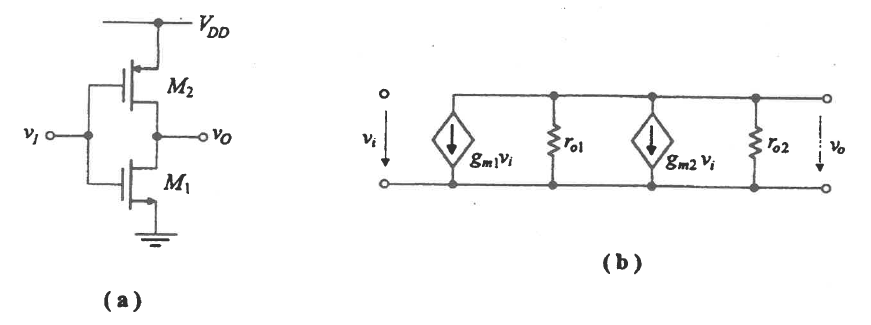
\includegraphics[width=0.6\linewidth]{img/5/inv-CMOS.png}
    \caption{Inversor CMOS \cite{medeiros:CTBM}}
    \label{fig:inv-CMOS}
\end{figure}

\vspace{-0.75em}
\noindent O funcionamento como inversor resume-se da seguinte forma (interruptores):
\begin{itemize}[leftmargin=*, nolistsep, label=\raisebox{-0.1em}{\ding{43}}]
    \item $v_I \to \text{HIGH}$, $M_1$ está na região de tríodo e $M_2$ está cortado, ficando $v_O = 0$;
    \item $v_I \to \text{LOW}$, $M_2$ está na região de tríodo e $M_1$ está cortado, e $v_O = V_{DD}$.
\end{itemize}

\begin{mdframed}
    \noindent Quando o circuito funciona como amplificador, $M_1$ e $M_2$ estão saturados, e o ganho de tensão é: $A_v = v_o/v_i = -(g_{m1} + g_{m2}) (r_{o1} // r_{o2})$.
    
    \vspace{0.5em}
    \noindent Este ganho tem um valor elevado, mas o circuito não se costuma utilizar muito como amplificador linear; prefere-se o andar de fonte comum com carga ativa, cujo ganho é da mesma ordem, mas o dimensionamento obedece a menos restrições.
\end{mdframed}

\iffalse
\newpage
\noindent O \textbf{inversor CMOS} tem características ótimas para funcionamento como circuito digital: a amplitude da saída é máxima, pois $v_O = 0$ ou $v_O = V_{DD}$ as características de transferência têm elevada inclinação na zona de transição (ganho de tensão elevado com os dois transístores saturados); nos dois estados de funcionamento a energia consumida pelo circuito é nula, pois não há corrente. A \textbf{potência estática}, dissipada pelo circuito quando permanece no mesmo estado, é nula. No entanto, quando o circuito muda de estado, há energia dissipada, uma vez que há passagem de corrente para carregar as capacidades parasitas e, por isso, a \textbf{potência dinâmica} não é nula.

Se considerarmos um condensador $C$ na saída do inversor, quando $v_O$ passa de $0$ para $V_{DD}$ o condensador recebe uma energia
$$
    W_e = C\,V_{DD}
$$
e a fonte de alimentação fornece uma energia
$$
    W_B = \int V_{DD}\, i_D\, dt = V_{DD} \int i_D\, dt = V_{DD}\, Q = V^2_{DD}C
$$
em que $Q = CV_{DD}$ é a carga fornecida pela fonte de alimentação ao condensador. A diferença entre a energia fornecida pela fonte e a energia que fica armazenada no condensador é a energia dissipada no circuito,
$$
    W_D = \frac{1}{2} C V^2_{DD}
$$
Da energia fornecida pela bateria, metade é dissipada no circuito e a outra metade é armazenada no condensador. Quando o circuito muda de estado e $v_O$ passa de $V_{DD}$ para $0$, a energia armazenada no condensador é dissipada no circuito. Deste modo, a energia $W_B$, fornecida pela bateria acaba por ser toda dissipada. Se o circuito funcionar como inversor lógico com um sinal de frequência $f$, a energia $W_B$ é dissipada $f$ vezes por unidade de tempo, e a \textbf{potência dinâmica} é
$$
    P = f C V^2_{DD}
$$
\fi

%//==============================--@--==============================//%
\subsection[5.2 Conceitos sobre Circuitos Digitais]{\hspace*{0.075 em}\raisebox{0.2 em}{$\pmb{\drsh}$} Conceitos sobre Circuitos Digitais}

Nos circuitos digitais, os sinais são binários, podendo ter dois valores lógicos, designados por 0 e 1. Os sinais são representados por tensões que podem ter nível alto, \textbf{H}, ou nível baixo, \textbf{L} (não é usual representar os sinais por correntes). Se ao nível alto se fizer corresponder o valor lógico 1 e ao nível baixo o valor lógico 0, diz-se que tem \textbf{lógica positiva}, que é a adotada nesta UC.

\begin{mdframed}
    \noindent Os circuitos digitais podem ser projetados e fabricados de maneiras distintas:
    \begin{itemize}[leftmargin=*, label=\rule{0.9ex}{0.9ex}]
        \item Se o volume de produção for baixo, ligam-se num circuito impresso os blocos necessários, disponíveis em embalagens separadas, cada uma com um circuito integrado de uso geral.
        
        \item Uma aplicação de volume elevado pode justificar a realização de um circuito integrado de aplicação espefícica, ou ASIC (\textit{Application Specific Integrated Circuit}), que é usualmente referido como circuito VLSI (\textit{Very Large Scale Integration}). Estes circuitos podem ser fabricados \textit{full-custom}, através do silício, se se justificar, ou com conjuntos de portas lógicas ou transístores (\textit{gate-arrays}), que são ligados pelo fabricante de acordo com as intruções do utilizador (\textit{semi-custom}).

        \item Existem circuitos deste género que podem ser diretamente programados pelo utilizador, denominados por FPGAs (\textit{Field Programmable Gate Arrays}).
    \end{itemize}
\end{mdframed}

\vspace{-1.0em}
\begin{figure}[H]
    \centering
    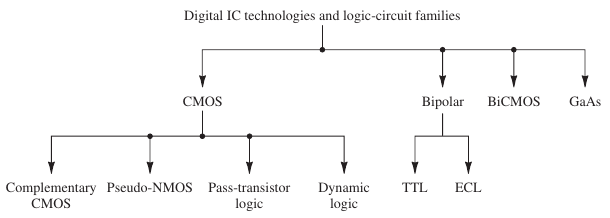
\includegraphics[width=0.6\linewidth]{img/5/logic-families.png}
    \caption{``Digital IC technologies and logic-circuit families.''\cite{sedra-smith:microelectronic-circuits}}
    \label{fig:logic-families}
\end{figure}

\vspace{-0.5em}
\noindent Os circuitos digitais agrupam-se em \textbf{famílias lógicas}, constituídas por circuitos com configuração semelhante, realizados com a mesma tecnologia e as mesmas características básicas. As principais famílias lógicas MOS são as NMOS (apenas se usa atualmente na realização de alguns ASIC e memórias) e CMOS; para os BJT, as principais famílias são as TTL (\textit{Transistor-Transistor Logic}) e a ECL (\textit{Emitter-Coupled Logic}). 

As três famílias: CMOS, TTL e ECL, são usadas para circuitos integrados de uso geral ou ASICs. 
\vspace{1em}\hrule\vspace{1em}
\noindent O circuito lógico mais elementar é o \textbf{inversor}. A maioria das características básicas das famílias lógicas pode ser estabelecida com base no inversor respetivo.

\begin{figure}[H]
    \centering
    \begin{minipage}[t]{0.16\linewidth}\vspace{0pt}%
        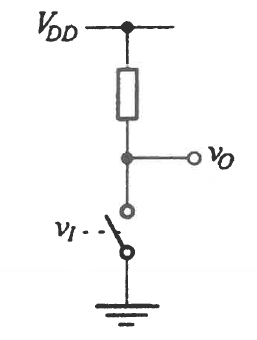
\includegraphics[width=\linewidth]{img/5/inverter.png}
        \caption{}
        \label{fig:inverter}
    \end{minipage}\hfill
    \begin{minipage}[t]{0.82\linewidth}\vspace{0pt}%
        A realização de um inversor baseia-se na utilização de um interruptor comandado. Quando a tensão de entrada $v_I$ tem nível alto, o interruptor fecha, e a tensão de saída $v_O$ fica no nível baixo. Quando $v_I$ está no nível baixo, o interruptor abre e $v_O$ fica no nível alto, dado que a saída fica ligada ao terminal positivo da alimentação através do dispositivo de carga (que sendo responsável pela subida de $v_O$, se designa por dispositivo de \textit{pull-up}; o interruptor comandado é o dispositivo de \textit{pull-down}).

        O interruptor comandado é um transístor e o dispositivo de carga pode ser uma resistência ou um transístor, como vimos na secção anterior.
    \end{minipage}
\end{figure}

\newpage
\noindent Nas especificações apresentadas pelos fabricantes para caracterizar as famílias lógicas, são indicados os seguintes níveis de tensão (considerando o \textbf{caso mais desfavorável}):

\begin{itemize}[leftmargin=*, label=]
    \item $V_{OH}$ --- tensão de saída mínima no estado 1;
    \item $V_{OL}$ --- tensão de saída máxima no estado 0;
    \item $V_{IH}$ --- tensão de entrada mínima que é sempre interpretada como 1;
    \item $V_{IL}$ --- tensão de entrada máxima que é sempre interpretada como 0;
\end{itemize}

\noindent $V_{IH}$ e $V_{IL}$ costumam considerar-se como os valores de $v_I$ para os quais a característica de transferência $v_O(v_I)$ tem declive -1.

\vspace{-0.75em}
\begin{figure}[H]
    \centering
    \begin{subfigure}[b]{0.55\linewidth}
        \centering
        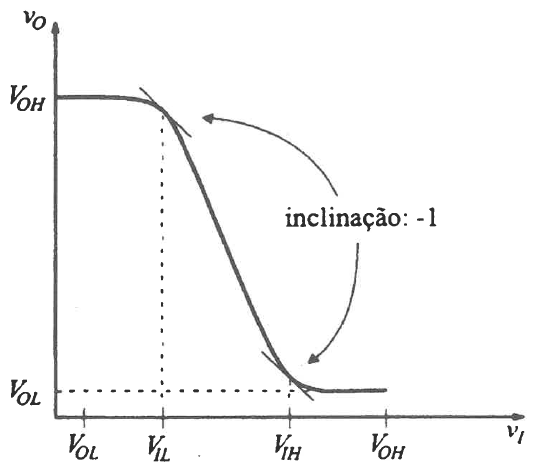
\includegraphics[width = \linewidth]{img/5/inv-transfer-function.png}
        \caption{Característica de transferência de um inversor real \cite{medeiros:CTBM}}
        \label{fig:inv-transfer-function}
    \end{subfigure}%%
    \begin{subfigure}[b]{0.3\linewidth}
        \centering
        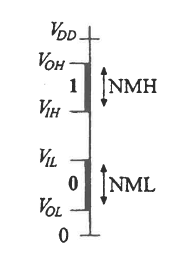
\includegraphics[width = 0.85\linewidth]{img/5/noise-margins.png}
        \caption{Margens de ruído \cite{medeiros:CTBM}}
        \label{fig:noise-margins}
    \end{subfigure}
    \caption{}
\end{figure}

\vspace{-0.75em}
\noindent Mesmo que um sinal tenha ruído sobreposto, desde que se situe entre $V_{IH}$ e $V_{OH}$ é sempre interpretado como 1; se se situar entre $V_{IL}$ e $V_{OL}$ será interpretado como 0.

\begin{mdframed}
    Por isso definem-se as \textbf{margens de ruído como}:
    $$\begin{aligned}
        \text{NM}_\text{H} &\delequal V_{OH} - V_{IH} \\
        \text{NM}_\text{L} &\delequal V_{IL} - V_{OL}
    \end{aligned}$$
    \noindent Interessa, naturalmente, que as margens de ruído sejam maximizadas.
\end{mdframed}

\noindent A saída de um circuito digital é, normalmente, ligada a uma ou mais entrada de outros circuitos da mesma família. Define-se como \textbf{leque de saída} (\textit{fan out}) ao número de entradas (de portas da mesma família lógica) que a saída de um circuito pode atuar, mantendo as caracteristicas especificadas pelo fabricante. Também se utiliza \textbf{leque de entrada} (\textit{fan in}) para designar o número de portas de entrada de uma porta lógica.

A \textbf{potência de dissipação} dos circuitos digitais constitui uma característica importante. Há que distinguir a \textbf{potência estática}, quando o circuito permanece num mesmo estado, e a \textbf{potência dinâmica}, que corresponde à energia dissipada quando o circuito muda de estado. A dissipação é normalmente diferente quando a saída está no estado 0 e quando está no estado 1. A potência estática é definida como a média da potência nos dois casos.

\noindent Os circuitos digitais não transitam de estados instantaneamente. Considerando os instantes de passagem pelo nível médio $(V_{OL} + V_{OH})/2$, há um atraso $t_{pHL}$ quando a saída passa do nível alto (H) para o nível baixo (L) e um atraso $t_{pLH}$ quando a saída faz a transição inversa. Define-se o \textbf{atraso de propagação} (\textit{propagation delay}) como
$$
    t_p = \frac{t_{pHL} + t_{pLH}}{2}
$$
\noindent \textbf{Nota:} Usualmente a corrente de carga é inferior à corrente de descarga, por isso
        $$
            t_{pLH} > t_{pHL}
        $$
\noindent (demora mais tempo a carregar do que a descarregar). 
        
\begin{figure}[H]
    \centering
    \begin{minipage}[t]{0.475\linewidth}\vspace{0pt}%
        \centering
        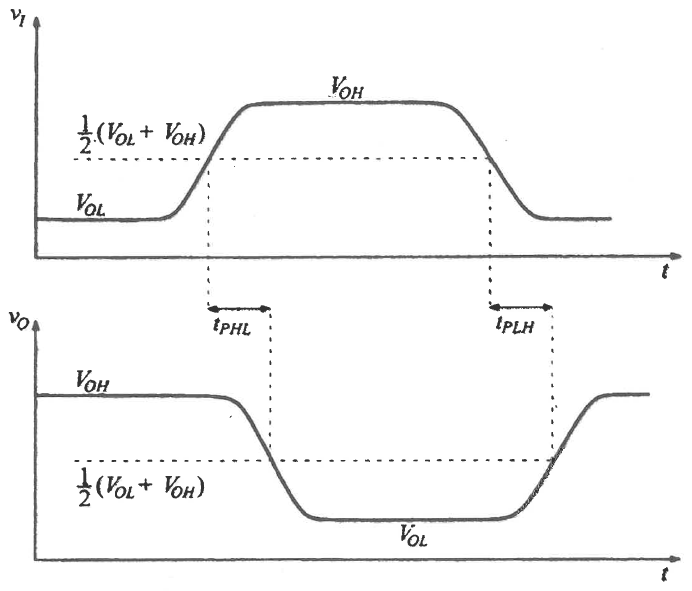
\includegraphics[width=1\linewidth]{img/5/propagation-delay.png}
        \caption{Atraso de propagação \cite{medeiros:CTBM}}
        \label{fig:propagation-delay}
    \end{minipage}\hfill%
    \begin{minipage}[t]{0.475\linewidth}\vspace{0pt}%
        Se $t_{pLH} \gg t_{pHL}$ então temos
        $$
            t_p \approx \frac{1}{2} t_{pLH}
        $$
        ``Nos circuitos digitais pretende-se rapidez de operação e baixo consumo, existindo um compromisso entre estes dois requisitos. As famílias lógicas costumam caracterizar-se pelo \textbf{produto atraso-potência}, $t_p P_D$ ($P_D$ é a potência estática média); interessa que o seu valor seja o menor possível.''\cite{medeiros:CTBM}
    \end{minipage}
\end{figure}

%//==============================--@--==============================//%
\subsection[5.3 Circuitos NMOS]{\hspace*{0.075 em}\raisebox{0.2 em}{$\pmb{\drsh}$} Circuitos NMOS}



%//==============================--@--==============================//%